% !TeX root = ../main.tex
% Add the above to each chapter to make compiling the PDF easier in some editors.

\chapter{Type Inference}\label{chapter:ti}
The previous chapter discusses the encoding of the type system in Z3. In this chapter, we explain how we build upon this encoding to provide a complete implementation for the static type inference.

\section{Type Inference Design}
We present here the main components of our type inference tool.
\subsection{Abstract Syntax Tree (AST)}
The AST of a program is a data structure which describes the structure of the source code, where each node in the tree represents a construct occurring in the program.

Figure \ref{fig:ast} shows a visualization for the AST of the Python program below.

\begin{lstlisting}
def f():
	return "Hello world!"
f()
\end{lstlisting}
\begin{figure}
	\begin{mdframed}
		\centering
		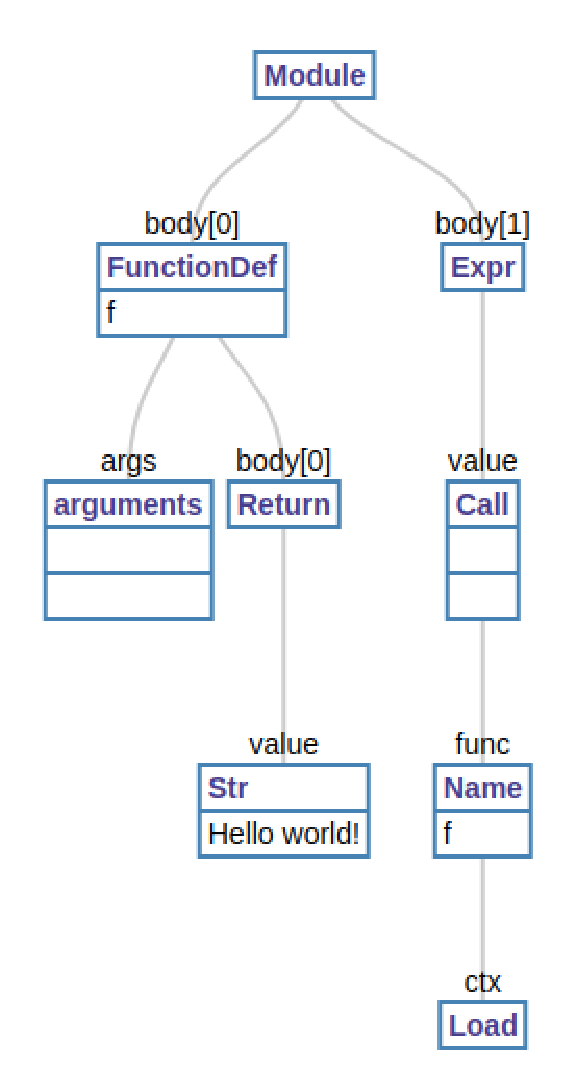
\includegraphics[width=50mm]{images/ast.eps}\\
	\end{mdframed}
	\caption{Abstract Syntax Tree (AST) for a Python program}
	\label{fig:ast}
\end{figure}

Our type inference works by traversing the AST in a depth-first manner, and gathering constraints along the way.
\subsection{Pre-analysis}
Before we attempt to infer the types of the input Python program, some pre-analysis is needed to prepare the configurations of the type inference.

The pre-analyzer takes the AST of the input program and provides the following information:

\begin{itemize}
	\item The maximum length of tuples that appear in the input program.
	\item The maximum length of function arguments that appear in the program.
	\item A mapping from all user-defined classes to their corresponding attributes and methods. There are two kinds to these attributes: \textit{class-level attributes} and \textit{instance-level attributes}. Class-level attributes are those that are not specific to certain instances, and can be accessed with the class type itself, while instance-level attributes are those which are tied to the class instance during its instantiation or later on. For instance, the class \lstinline|A| in the following example has two attributes, namely \lstinline|x| and \lstinline|y|, where attribute \lstinline|x| is a class-level attribute while \lstinline|y| is an instance-level attribute.
	
	\begin{lstlisting}
class A:
	x = 1
	def __init__(self):
		self.y = 1
		
A.x  # valid
A().x  # valid
A().y  # valid
A.y  # invalid
	\end{lstlisting}
	
	Class-level attributes are detected by the pre-analyzer whenever it encounters an assignment statement in the top-level scope of the class in which the left-hand side is a normal variable.
	
	Instance-level attributes are recognized whenever they are assigned by accessing the first argument in the class methods, like accessing \lstinline|self| argument in the above example.
	
	Class-level attributes represent a subset of the instance-level attributes, that is every instance of a certain class can access any class-level attribute. However, instance-level attributes cannot be accessed by the class type itself.
	
	\item A mapping from all user-defined classes to their base classes if they have any.
	\item The inheritance DAG which is used to generate the subtyping constraints discussed in the previous chapter.
\end{itemize}

In addition to the above information, the pre-analyzer also does the following pre-processing to the user-defined classes:
\begin{itemize}
	\item Adds a default \lstinline|__init__| method to classes which do not contain one.
	
	This default \lstinline|__init__| method has the following source:
	\begin{lstlisting}
def __init__(self):
	pass
	\end{lstlisting}
	\item Propagates methods and attributes from base classes to their subclasses. The method resolution order which governs the order of this propagation is discussed later in this chapter.
\end{itemize}

\subsection{Context Hierarchy}
A context contains the information that a certain scope in the program holds. It contains a mapping from the variable names in this context to the Z3 variables representing their types, which are evaluated to the correct types after solving the SMT problem. Every context also has references to its children contexts (which are created inside the scope of this context) and a reference to its parent context.

Below is a listing of the constructs which create new contexts:

\begin{itemize}
	\item \lstinline|if| statements.
	\item \lstinline|for| and \lstinline|while| loops.
	\item Function definitions
	\item Class definitions
	\item List, set and dictionary comprehensions
\end{itemize}

Figure \ref{fig:contexts} shows a tree representing the context hierarchy for the Python program below.

\begin{figure}[H]
	\begin{mdframed}
		\Tree[.{global} [.{A} {f} {g} ] [.{for} {if} {else} ] {list comp} ]
	\end{mdframed}
	\caption{Context hierarchy for a Python program}
	\label{fig:contexts}
\end{figure}

\begin{lstlisting}
x = [1, 2, 3]

class A:
	def f(self):
		pass
	def g(self):
		pass
	
for i in x:
	if True:
		pass
	else:
		pass
		
y = [i + 1 for i in x]
\end{lstlisting}
\subsection{Z3 Solver}
The Z3 solver is the main component in the type inference design. It is responsible for solving all the constraints imposed by the Python program semantics, or report that they are impossible to be satisfied.

We extend the default solver in Z3, such that during the instantiation of every solver instance, the following takes place:

\begin{itemize}
	\item The pre-analysis defined above in processed.
	\item The \textit{type sort} data-type is declared with all its constructors.
	\item The subtyping rules discussed in chapter \ref{chapter:background} are initialized. 
\end{itemize}

At the end of the program inference, this solver is queried for a solution to all the added constraints.

\subsection{Import Handler}
As the name suggests, the import handler is responsible for handling module importing during the type inference.

If the imported module is a built-in Python package, it retrieves the module from the corresponding stub file and infers the types of its contents, otherwise, it reads the imported module from the disk and infers its types in a separate context.\\

We will discuss later in this chapter different types of import statements in Python and how they are handled in our type inference.
\subsection{Stubs Handler}
As discussed earlier, \textbf{stubs} are files containing code which simulates built-in functionalities. A \textbf{stub function} is a function declaration which mocks some other function. The following function is a stub function which mocks the built-in function \lstinline|len|:

\begin{lstlisting}
def len(_: object) -> int:
	...
\end{lstlisting}

Stubs enable the type inference to infer the types of programs using built-ins. The stubs handler is the module responsible for organizing the relevant stub files which are required by the program being inferred.
\subsection{Inference Configuration}
The user of the type inference has the ability to control the behavior of the type inference according to some pre-defined configurations. Each configuration is expected to have its gain and limitation. Some configurations, for instance, lead to a significant increase in the inference speed, yet at the cost of rejecting a larger set of correct programs. We will discuss the current possible configurations when we get to the rules related to these configurations.
\subsection{Hard Constraints vs. Soft Constraints}
An important addition to our type inference was introducing the ability to add soft constraints. \textbf{Hard constraints} are the constraints that \textbf{must} be satisfied by the program, such that if at least one hard constraint cannot be satisfied, the program is rejected and cannot type. On the other hand, \textbf{soft constraints} are those that are good to be satisfied, but they are not obligatory, such that a program violating some soft constraints is not rejected by the type inference. See the following example for illustration:

\begin{lstlisting}
def f(x):
	y = [1, 2, 3]
	return y[x]
\end{lstlisting}

Here, the array \lstinline|y| is indexed with variable \lstinline|x|. Therefore, the type of \lstinline|x| \textbf{must} be a subtype of \lstinline|int|, so a program in which the type of \lstinline|x| violates this constraint (e.g., having \lstinline|x| as a float) would be rejected. The constraint in this case is a hard one. Another hard constraint is added in the assignment statement \lstinline|y = [1, 2, 3]|, that the type of the array literal \lstinline|[1, 2, 3]| is a subtype of the type of variable \lstinline|y|. Moreover, a soft constraint is added that both the type of the array literal and the type of \lstinline|y| are the same. Without this soft constraint, the type of \lstinline|y| in the model given by Z3 might be an \lstinline|object|, or any super type of the right-hand side (which is correct and sound, but not very accurate). So the purpose of the hard constraints is to provide a sound type inference, while that of the soft constraints is to increase its accuracy.
\section{Type Inference Rules}
Having explained the main components of the type inference, we are now ready to discuss the axioms added for every construct in the Python program.
\subsection{Expressions Axioms}
\subsection{Statements Axioms}
\subsection{Function Definitions Inference}
\subsection{Class Definitions Inference}
\subsection{Function Calls and Class Instantiation Inference}
\subsection{Attribute Access}
\subsection{Module Importing}

\section{Inference Output}
\subsection{Typed AST}
\subsection{Error Reporting}